\documentclass[11pt,letterpaper]{article}
%\documentstyle[11pt]{article}
\usepackage[utf8]{inputenc}
\usepackage{amsmath}
\usepackage{xfrac}
\usepackage{amsfonts}
\usepackage{amssymb}
\usepackage[version = 3]{mhchem}
\usepackage{chemstyle}
\usepackage{graphicx}
\usepackage{epstopdf}
%\usepackage{tabularx,ragged2e,booktabs,caption}
%\newcolumntype{C}[1]{>{\Centering}m{#1}}
%\renewcommand\tabularxcolumn[1]{C{#1}}
%\usepackage[left=2cm,right=2cm,top=2cm,bottom=2cm]{geometry}
\usepackage{subcaption} 
\usepackage{caption}
\usepackage[left=2cm,right=2cm,top=1cm,bottom=2cm]{geometry}
%\usepackage{siunitx}



\begin{document}
\setlength{\parindent}{0cm} 



\frenchspacing

% Default margins are too wide all the way around. I reset them here
%\setlength{\topmargin}{-.5in}
%\setlength{\textheight}{9in}
%\setlength{\oddsidemargin}{.125in}
%\setlength{\evensidemargin}{.125in}
\setlength{\textwidth}{6.25in}

\title {\Large{\textbf{Mass Balance on Reservoir and Irrigated Farmland}}\\ \large{CENG 340--Introduction to Environmental Engineering\\
Instructor: Deborah Sills\\ \textbf{In Class: October 4, 2013}}}

\author {}
\date {}
\maketitle

\vspace{-1.5cm}
As illustrated in the figure below, a river flows into a reservoir that is being used to irrigate farmland.  The river inflow is 30,000 $\mathrm{\frac{m^3}{yr}}$ and the salt concentration in the river is 300 $\mathrm{\frac{g}{m^3}}$.  The reservoir can be modeled as being \emph{completely mixed} with a uniform salt concentration.\\

The farmland needs irrigation water to flush salts out of the soil and for use by plants.  Water used by plants is lost by evapotranspiration and the net amount of this loss over and above the water input from rainfall, Q$\mathrm{_E}$, equals 10,000 $\mathrm{\frac{m^3}{yr}}$.\\

Salty water from the farm is returned to the reservoir.  The salt concentration in the return flow is 2,500 $\mathrm{\frac{g}{m^3}}$.\\

You may assume that the whole system is at steady state with unchanging flows and constant salt concentrations in the river, the agricultural return flow, and the reservoir.\\

Find:
\begin{enumerate}
\item the flow out of the reservoir, Q$\mathrm{_{out}}$.
\item the salt concentration in the reservoir, which is the same as the concentration in the flow out of the reservoir (since the reservoir is completely mixed).
\item the flow rate for the irrigation water, Q$\mathrm{_{irr}}$.  Note that this is different from the rate of the return flow.

\end{enumerate}

\begin{figure}
\centering
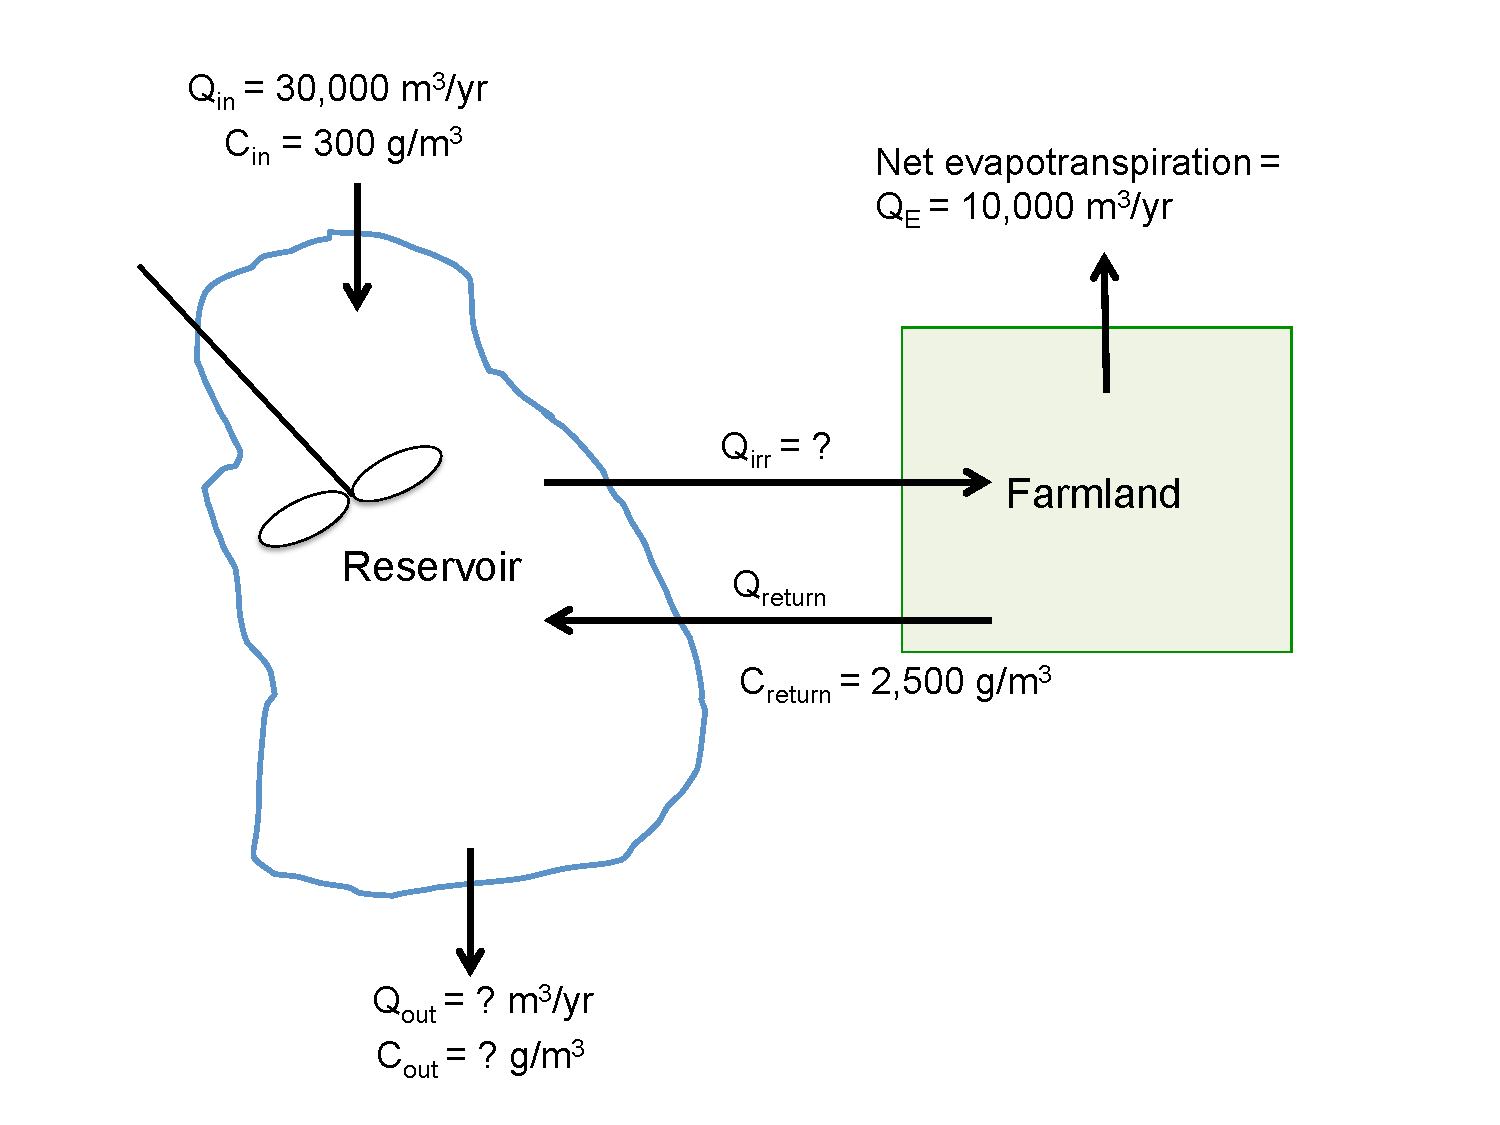
\includegraphics[width=0.7\textwidth]{massbalance_farm}
\end{figure}




\end{document}